% ══════════════════════════════════════════════════════════════════════
% IEEE TNNLS Journal Paper
% Continual Learning and Constrained Reinforcement Learning for
% Adversarially Robust Network Intrusion Detection and Response
% ══════════════════════════════════════════════════════════════════════
\documentclass[journal]{IEEEtran}

% ── Packages ─────────────────────────────────────────────────────────
\usepackage[T1]{fontenc}
\usepackage[utf8]{inputenc}
\usepackage{amsmath,amssymb,amsthm}
\usepackage{mathtools}
\usepackage{graphicx}
\usepackage{booktabs}
\usepackage{multirow}
\usepackage{tabularx}
\usepackage{xcolor}
\usepackage{pifont}
\usepackage{cite}
\usepackage{balance}
\usepackage{algorithm}
\usepackage{algorithmic}
\usepackage{tikz}
\usetikzlibrary{arrows.meta,positioning,shapes.geometric,calc,fit,backgrounds}
\usepackage{pgfplots}
\pgfplotsset{compat=1.18}
\usepackage{subcaption}
\usepackage{url}
\usepackage[colorlinks=true,citecolor=blue!60!black,linkcolor=blue!60!black,urlcolor=blue!50!black]{hyperref}
\usepackage{threeparttable}

% ── Theorem environments ─────────────────────────────────────────────
\theoremstyle{definition}
\newtheorem{definition}{Definition}
\newtheorem{problem}{Problem}
\theoremstyle{remark}
\newtheorem{remark}{Remark}

% ── Custom commands ──────────────────────────────────────────────────
\newcommand{\RobustIDPS}{\textsc{RobustIDPS.ai}}
\newcommand{\EWC}{\textsc{EWC}}
\newcommand{\CPO}{\textsc{CPO}}
\newcommand{\PPO}{\textsc{PPO}}
\newcommand{\CMDP}{\textsc{CMDP}}
\newcommand{\FIM}{\mathbf{F}}
\newcommand{\loss}{\mathcal{L}}
\newcommand{\expect}{\mathbb{E}}
\newcommand{\real}{\mathbb{R}}
\DeclareMathOperator*{\argmax}{arg\,max}
\DeclareMathOperator*{\argmin}{arg\,min}

% ═════════════════════════════════════════════════════════════════════
\begin{document}

\title{Continual Learning and Constrained Reinforcement Learning for Adversarially Robust Network Intrusion Detection and Autonomous Response}

\author{Roger~Nick~Anaedevha,~\IEEEmembership{Student~Member,~IEEE,}
        Alexander~Gennadievich~Trofimov,
        and~Yuri~Vladimirovich~Borodachev%
\thanks{R.\,N.~Anaedevha and A.\,G.~Trofimov are with the Institute
of Cyber-Intelligent Systems (ICIS), National Research Nuclear University
MEPhI, Moscow 115409, Russian Federation
(e-mail: roger@robustidps.ai; agtrofimov@mephi.ru).}%
\thanks{Y.\,V.~Borodachev is with the Department of Applied Mathematics,
National Research Nuclear University MEPhI, Moscow 115409,
Russian Federation (e-mail: yvborodachev@mephi.ru).}%
\thanks{Manuscript submitted March 2026.}}

\markboth{IEEE Transactions on Neural Networks and Learning Systems}%
{Anaedevha \MakeLowercase{\textit{et al.}}: Continual Learning and Constrained RL for Adversarially Robust NIDS}

\maketitle

% ═════════════════════════════════════════════════════════════════════
% ABSTRACT
% ═════════════════════════════════════════════════════════════════════
\begin{abstract}
Machine-learning-based network intrusion detection systems achieve high accuracy under static conditions, yet two fundamental limitations impede their operational deployment. First, fixed-weight classifiers degrade as network traffic distributions evolve, a phenomenon known as concept drift, and naive retraining risks catastrophic forgetting of previously learned attack signatures. Second, detection without automated response leaves a critical gap between identification and mitigation, one that human analysts cannot bridge at the scale and speed required by modern networks. This paper presents a unified framework that addresses both limitations simultaneously. The detection component employs Elastic Weight Consolidation combined with experience replay to enable incremental adaptation of a seven-branch surrogate ensemble across sequential traffic distributions, bounding accuracy regression on any previously learned attack class to fewer than two percentage points. The response component formulates automated mitigation as a Constrained Markov Decision Process and trains a policy via Constrained Policy Optimisation that selects graduated response actions, from passive monitoring through connection reset to full quarantine, while provably bounding the false-positive blocking rate below 0.1\%. Both components share the Fisher Information Matrix as a unifying mathematical object: for knowledge preservation in the continual learning module and for trust-region constraint satisfaction in the policy optimiser. Comprehensive experiments across six benchmark datasets comprising 84.2 million flow records and 83 unique attack classes demonstrate that the proposed method maintains 96.9\% average accuracy under sequential task learning, reduces backward transfer (forgetting) to $-0.014$ compared with $-0.153$ for naive fine-tuning, and achieves a 97.2\% threat mitigation rate with zero safety constraint violations over 5{,}000 evaluation episodes. The integrated system, deployed on the \RobustIDPS{} production platform, processes live network traffic with sub-second detection-to-response latency, representing the first closed-loop intrusion detection and response system that simultaneously addresses continual adaptation, adversarial robustness, and formally constrained autonomous action.
\end{abstract}

\begin{IEEEkeywords}
Continual learning, reinforcement learning, network intrusion detection, constrained Markov decision process, Elastic Weight Consolidation, adversarial robustness, Fisher Information Matrix, autonomous cyber defence.
\end{IEEEkeywords}

% ═════════════════════════════════════════════════════════════════════
% I. INTRODUCTION
% ═════════════════════════════════════════════════════════════════════
\section{Introduction}
\label{sec:intro}

\IEEEPARstart{N}{etwork} intrusion detection systems (NIDS) constitute a foundational layer in modern enterprise security architectures. Traditional signature-based systems, notably Suricata and Snort, depend on manually curated rule sets that cannot generalise to novel attack variants. Machine-learning-based alternatives have demonstrated substantially higher detection rates across diverse traffic corpora, yet they introduce a limitation of a different kind: once trained, their model parameters remain frozen. In production environments, network traffic distributions evolve continuously as new application protocols emerge, user behaviour shifts, and adversaries adapt their tactics. This phenomenon, widely termed concept drift~\cite{gama2014survey}, causes the accuracy of fixed-weight classifiers to degrade over time, sometimes precipitously. Amalapuram~\textit{et~al.}\ observed that without continual adaptation, attack-class precision--recall area under the curve can decline from 0.985 to 0.506 within as few as three days of deployment~\cite{amalapuram2024soul}.

Periodic full retraining offers a brute-force remedy but carries significant operational costs. It is computationally expensive, requires access to the full historical dataset, and risks introducing regressions on previously well-classified attack families. More critically, gradient-based retraining on new data tends to overwrite parameters that encode knowledge of earlier tasks, a well-documented pathology known as catastrophic forgetting~\cite{kirkpatrick2017ewc}. Continual learning, the paradigm in which a model learns sequentially from a stream of tasks $\mathcal{T}_1, \mathcal{T}_2, \ldots, \mathcal{T}_T$ while retaining performance on all prior tasks, addresses precisely this challenge. Among continual learning methods, Elastic Weight Consolidation (EWC) has proven effective in constraining parameter drift by penalising changes to weights deemed important for previous tasks, as quantified by the diagonal of the Fisher Information Matrix (FIM)~\cite{kirkpatrick2017ewc}. When combined with experience replay, in which a bounded memory buffer of representative past samples is interleaved with current training data, EWC achieves a favourable balance between stability and plasticity~\cite{amalapuram2023augmented}.

Concurrently, detection without response constitutes only half the defensive mission. Current systems generate alerts that human analysts must triage manually, a bottleneck that becomes untenable at the scale of modern network telemetry. An autonomous response capability that selects and executes mitigation actions---subject to configurable safety constraints---would close the loop between detection and remediation. Reinforcement learning (RL) provides a natural framework for this sequential decision problem, and constrained Markov decision processes (CMDPs)~\cite{altman1999constrained} extend the standard RL formulation with explicit cost constraints that bound unsafe behaviour. Constrained Policy Optimisation (CPO)~\cite{achiam2017cpo}, which solves the CMDP objective through trust-region updates, offers a principled mechanism for ensuring that automated mitigation actions remain within operationally acceptable bounds.

A key observation motivating the present work is that both EWC and CPO rely on the same mathematical object---the Fisher Information Matrix---but for complementary purposes. In the continual learning module, the FIM quantifies the importance of each parameter for previously learned tasks, enabling selective knowledge preservation. In the policy optimiser, the FIM defines the trust region within which policy updates satisfy safety constraints. This duality, which to the best of our knowledge has not been exploited in prior work, suggests a unified computational framework in which a single FIM computation serves both continual adaptation and constrained response.

In our earlier work, we developed a stochastic multimodal transformer with uncertainty quantification that forms the detection backbone of the \RobustIDPS{} platform~\cite{anaedevha2026stochastic}. Subsequent studies introduced MambaShield, a selective state-space architecture resilient to data poisoning attacks~\cite{anaedevha2026mambashield}, and uncertainty-calibrated hierarchical Gaussian processes for multi-scale temporal modelling of network flows~\cite{anaedevha2026gp}. Together, these contributions established the adversarially robust, uncertainty-aware detection infrastructure upon which the present continual learning and autonomous response modules are built.

The contributions of this paper are fourfold. First, we design and implement a continual learning pipeline that combines EWC regularisation with reservoir-sampled experience replay, enabling incremental updates to a seven-branch surrogate ensemble while bounding forgetting to fewer than two percentage points on any previously encountered attack class (Section~\ref{sec:method}). Second, we formulate the automated response problem as a CMDP with graduated action severity and train a CPO-based agent whose false-positive blocking rate is formally bounded below 0.1\% (Section~\ref{subsec:rl_method}). Third, we unify both modules through shared FIM computation, reducing the computational overhead of maintaining separate importance matrices for continual learning and policy trust regions (Section~\ref{subsec:unified_fim}). Fourth, we conduct extensive experiments across six benchmark datasets totalling 84.2~million flow records and 83 unique attack classes, demonstrating state-of-the-art performance in sequential adaptation, response effectiveness, and adversarial robustness (Section~\ref{sec:results}).

The remainder of this paper is organised as follows. Section~\ref{sec:related} reviews related work in continual learning for NIDS, reinforcement learning for autonomous cyber defence, and adversarial robustness. Section~\ref{sec:problem} formalises the problem and identifies specific gaps in the existing literature. Section~\ref{sec:method} details the proposed methodology, including the continual learning pipeline, the constrained RL agent, and their integration through shared Fisher information. Section~\ref{subsec:exp_setup} describes the experimental design, and Section~\ref{sec:results} presents the results. Section~\ref{sec:discussion} discusses the implications, limitations, and directions for future research, and Section~\ref{sec:conclusion} concludes.

% ═════════════════════════════════════════════════════════════════════
% II. RELATED WORK
% ═════════════════════════════════════════════════════════════════════
\section{Related Work}
\label{sec:related}

This section surveys three research streams whose intersection defines the scope of the present paper: continual learning for network intrusion detection, reinforcement learning for autonomous cyber defence, and adversarial robustness of machine-learning-based NIDS. Each stream has matured considerably since 2022, yet as we shall demonstrate in Section~\ref{sec:problem}, no existing work integrates all three into a unified framework.

\subsection{Continual Learning for Network Intrusion Detection}
\label{subsec:cl_related}

The continual learning literature is broadly organised into three families. Regularisation methods, exemplified by EWC~\cite{kirkpatrick2017ewc}, Synaptic Intelligence~\cite{zenke2017continual}, and Memory Aware Synapses~\cite{aljundi2018memory}, add a penalty to the loss that discourages modifications to parameters deemed important for prior tasks. Replay methods maintain an episodic memory of past samples and interleave them during training; Gradient Episodic Memory (GEM)~\cite{lopezpaz2017gem} and its efficient variant A-GEM~\cite{chaudhry2019agem} additionally constrain gradient directions to avoid increasing the loss on stored exemplars. Architecture methods allocate dedicated capacity for each task, either by growing the network progressively~\cite{rusu2016progressive} or by masking weight subsets~\cite{serra2018overcoming}.

Application of these methods to intrusion detection has accelerated in recent years. Amalapuram~\textit{et~al.}~\cite{amalapuram2023augmented} introduced an augmented memory replay approach combining Extended Class Balancing Reservoir Sampling (ECBRS) with Perturbation Assistance for Parameter Approximation (PAPA), demonstrating 12--40\% training time savings over Maximally Interfered Retrieval (MIR) across six NIDS benchmarks at NeurIPS~2023. Their earlier foundational work established that rehearsal-based methods consistently match upper-bound performance on NIDS tasks while EWC and Synaptic Intelligence struggle under severe class imbalance, the defining challenge of network traffic datasets~\cite{amalapuram2022comsnets}. The SPIDER framework~\cite{amalapuram2024spider}, presented at IEEE INFOCOM~2024, demonstrated that combining Gradient Projection Memory with semi-supervised learning achieves comparable performance to fully supervised baselines using only 20\% annotated data, while its successor SOUL~\cite{amalapuram2024soul} extended this to open-world scenarios where novel attack classes appear without prior knowledge.

More recent contributions have addressed specific aspects of the continual NIDS problem. Zhang~\textit{et~al.}~\cite{zhang2025ssf} proposed Strategic Selection and Forgetting (SSF), accepted at IEEE~INFOCOM~2025, which uses KL-divergence-based drift detection to selectively discard outdated knowledge that actively hinders adaptability. EL-GNN~\cite{elgnn2025} integrated EWC into graph neural networks for task-incremental IDS, achieving 95.9\% accuracy on CIC-IDS-2017 in continual settings. CND-IDS~\cite{cndids2025} demonstrated a 6.1$\times$ F-score improvement over unsupervised continual learning baselines through PCA-based novelty detection, enabling zero-day attack identification without labelled attack data.

Despite these advances, a persistent limitation of all existing continual NIDS approaches is their exclusive focus on detection. None incorporates an automated response mechanism, leaving the critical gap between identifying a threat and acting upon it entirely to human operators. Addressing this gap requires the reinforcement learning methods surveyed in the following subsection.

\subsection{Reinforcement Learning for Autonomous Cyber Defence}
\label{subsec:rl_related}

The application of RL to automated cyber defence has gained traction through standardised simulation environments and competitive challenges. CyberBattleSim~\cite{msdefender2021cyberbattlesim} provides a graph-based network simulation for attacker-defender games, while the Cyber Autonomy Gym for Experimentation (CAGE) Challenge series~\cite{cage2022,kiely2025cage4} has established the primary benchmark for autonomous cyber defence research. Foley~\textit{et~al.}~\cite{foley2022cage2} won CAGE Challenge~2 using hierarchical Proximal Policy Optimisation (\PPO{}) to defend 13~hosts across three subnets, and Singh~\textit{et~al.}~\cite{singh2025hmarl} advanced the state of the art at CAGE Challenge~4 with Hierarchical Multi-Agent RL (H-MARL) for defending an 18-drone ad~hoc network. Additional environments including Yawning Titan~\cite{andrew2022yawningtitan}, CybORG++~\cite{cyborgpp2024}, and Cyberwheel~\cite{cyberwheel2024} provide increasingly sophisticated training testbeds.

Several recent works have explored novel RL architectures for cyber defence. Entity-based RL~\cite{symes2024entity} achieves zero-shot generalisation to unseen network topologies using Transformer-based \PPO{} policies trained in Yawning Titan. Causally Aware RL~\cite{purves2024causal} integrates causal inference with model-based RL for improved robustness across attacker skill levels. The Adaptive Reinforcement Learning for Cybersecurity Incident Response (ARCS) framework~\cite{arcs2025} reports 27.3\% faster incident resolution and 31.2\% higher defence effectiveness compared with rule-based baselines.

A critical gap in this literature concerns safety. Foundational safe RL methods exist---CPO~\cite{achiam2017cpo} provides near-constraint satisfaction guarantees through trust-region updates, PPO-Lagrangian~\cite{ray2019ppolag} converts CMDPs to unconstrained problems via dual gradient ascent, and Constrained Variational Policy Optimisation (CVPO)~\cite{liu2022cvpo} achieves 100--1000$\times$ fewer constraint violations in off-policy settings. Yet none of these has been applied to network cyber defence. All existing autonomous defence systems handle safety exclusively through reward shaping, an approach that provides no formal guarantees on operationally critical quantities such as false-positive blocking rates. The need for formal safety constraints in automated response provides the second motivation for the present work, and its integration with continual learning is addressed in Section~\ref{subsec:unified_fim}.

\subsection{Adversarial Robustness of Machine-Learning-Based NIDS}
\label{subsec:adv_related}

Machine-learning-based NIDS are vulnerable to adversarial manipulation at both inference time, through evasion attacks, and training time, through data poisoning~\cite{he2023advsurvey}. He~\textit{et~al.}~\cite{he2023advsurvey} established that computer-vision-based adversarial attack methods do not transfer directly to the network traffic domain owing to feature interdependency constraints: network flow features possess semantic relationships (non-negative integer packet counts, duration-bounded byte volumes) that restrict the attacker's feasible perturbation space. Nevertheless, domain-adapted attacks remain effective; decision-based black-box attacks achieve greater than 86\% success rates against most classifiers on NSL-KDD~\cite{sharma2024blackbox}.

Multi-strategy defences have demonstrated promising restoration of detection capability. TIKI-TAKA~\cite{zhang2022tikitaka} showed that combining model voting ensembles, ensemble adversarial training, and query detection restores detection rates to nearly 100\% against evasion attackers achieving up to 35.7\% success rate on CIC-IDS2017/2018. Tafreshian and Zhang~\cite{tafreshian2025defence} achieved a 35\% average increase in detection accuracy under adversarial conditions through integrated adversarial training, SMOTE balancing, and ensemble learning. MARS~\cite{mars2025} extended randomised smoothing certification to multiple $\ell_p$ norms for NIDS, providing the first framework with certified robustness guarantees in this domain.

Uncertainty quantification offers a complementary defence axis. Talpini~\textit{et~al.}~\cite{talpini2024uq} demonstrated that Bayesian neural networks provide superior out-of-distribution detection for open-set NIDS classification. Our prior work on uncertainty-calibrated hierarchical Gaussian processes~\cite{anaedevha2026gp} and stochastic multimodal transformers~\cite{anaedevha2026stochastic} established that principled uncertainty estimation enables the detection layer to communicate confidence to downstream decision systems. This communication channel is precisely what the RL response agent in the present work exploits: low-confidence detections trigger conservative actions, while high-confidence alerts enable more aggressive mitigation, a design enabled by the MambaShield architecture's resilience to poisoning-induced uncertainty degradation~\cite{anaedevha2026mambashield}.

State-space models have emerged as a promising architecture for sequential network traffic modelling. NetMamba~\cite{wang2024netmamba} achieves approximately 99\% accuracy across six traffic classification benchmarks with 60$\times$ faster inference than Transformer baselines. IDS-GraphMamba~\cite{idsgraphmamba2025} combines Mamba layers with Markov-chain graph aggregation for edge-network intrusion detection. However, no existing work evaluates the adversarial robustness of Mamba-based NIDS architectures, nor integrates state-space models within a continual learning pipeline---both directions that the present framework is designed to accommodate.

% ═════════════════════════════════════════════════════════════════════
% III. PROBLEM FORMULATION AND GAP ANALYSIS
% ═════════════════════════════════════════════════════════════════════
\section{Problem Formulation and Gap Analysis}
\label{sec:problem}

The preceding review reveals three independently maturing research streams that have not been integrated. This section formalises the individual sub-problems, identifies the precise gaps at their intersection, and motivates the unified formulation that the proposed method addresses.

\subsection{Continual Detection Under Distribution Shift}
\label{subsec:prob_cl}

Let $f_\theta : \mathcal{X} \to \Delta^{K}$ denote a neural network classifier parameterised by $\theta \in \real^d$ that maps a flow feature vector $\mathbf{x} \in \mathcal{X} \subseteq \real^n$ to a probability distribution over $K$ traffic classes, where $\Delta^K$ is the $K$-dimensional probability simplex. In a deployment environment, the classifier encounters a sequence of data distributions $\mathcal{D}_1, \mathcal{D}_2, \ldots, \mathcal{D}_T$, each representing a distinct temporal period during which the joint distribution $P(\mathbf{x}, y)$ may differ from that of previous periods.

\begin{definition}[Distribution Shift in Network Traffic]
\label{def:drift}
A distribution shift between periods $t$ and $t'$ occurs when $P_t(\mathbf{x}, y) \neq P_{t'}(\mathbf{x}, y)$, which may manifest as covariate shift ($P_t(\mathbf{x}) \neq P_{t'}(\mathbf{x})$ while $P(y|\mathbf{x})$ is stable), prior probability shift ($P_t(y) \neq P_{t'}(y)$), or concept shift ($P_t(y|\mathbf{x}) \neq P_{t'}(y|\mathbf{x})$).
\end{definition}

The continual learning objective is to find parameters $\theta^{(T)}$ after observing all $T$ distributions that maximise detection performance across all periods. We quantify this through three standard metrics. Average Accuracy (AA) is defined as $\mathrm{AA} = \frac{1}{T}\sum_{t=1}^{T} a_{T,t}$, where $a_{T,t}$ denotes the accuracy on task $t$ after training through task $T$. Backward Transfer (BWT) measures forgetting as $\mathrm{BWT} = \frac{1}{T-1}\sum_{t=1}^{T-1}(a_{T,t} - a_{t,t})$, where negative values indicate performance loss on earlier tasks. Forward Transfer (FWT) captures generalisation to future tasks as $\mathrm{FWT} = \frac{1}{T-1}\sum_{t=2}^{T}(a_{t,t} - \tilde{a}_t)$, where $\tilde{a}_t$ denotes the accuracy of a randomly initialised model on task $t$.

\begin{problem}[Continual Detection]
\label{prob:cl}
Given a sequence of labelled traffic datasets $\{(\mathcal{D}_t)\}_{t=1}^{T}$ arriving sequentially, find an update rule $\theta^{(t)} = \mathcal{U}(\theta^{(t-1)}, \mathcal{D}_t, \mathcal{B})$ that satisfies:
\begin{align}
&\text{(i)} \quad \mathrm{AA} \geq \mathrm{AA}_{\mathrm{retrain}} - \epsilon_{\mathrm{acc}}, \label{eq:cl_obj1}\\
&\text{(ii)} \quad \mathrm{BWT} \geq -\epsilon_{\mathrm{forget}}, \label{eq:cl_obj2}\\
&\text{(iii)} \quad \mathrm{Cost}(\mathcal{U}) \ll \mathrm{Cost}(\text{full retrain}), \label{eq:cl_obj3}
\end{align}
where $\mathcal{B}$ is a bounded replay buffer, $\epsilon_{\mathrm{acc}} = 0.02$, $\epsilon_{\mathrm{forget}} = 0.02$, and $\mathrm{AA}_{\mathrm{retrain}}$ is the accuracy of full retraining on the union of all observed data.
\end{problem}

Existing continual NIDS methods address Problem~\ref{prob:cl} through various combinations of replay and regularisation, but they produce only detection outputs. Converting these detections into effective mitigation requires the decision framework formalised next.

\subsection{Constrained Autonomous Response}
\label{subsec:prob_rl}

Given the detection outputs of the continual classifier, the response problem is to select mitigation actions that minimise expected damage while satisfying safety constraints. We formalise this as a CMDP.

\begin{definition}[Response CMDP]
\label{def:cmdp}
A Constrained Markov Decision Process is a tuple $(\mathcal{S}, \mathcal{A}, P, R, C, d_0, \gamma)$, where $\mathcal{S}$ is the state space, $\mathcal{A}$ the action space, $P: \mathcal{S} \times \mathcal{A} \times \mathcal{S} \to [0,1]$ the transition kernel, $R: \mathcal{S} \times \mathcal{A} \to \real$ the reward function, $C: \mathcal{S} \times \mathcal{A} \to \real$ a cost function encoding safety constraints, $d_0$ the initial state distribution, and $\gamma \in (0,1)$ the discount factor.
\end{definition}

The RL agent seeks a policy $\pi: \mathcal{S} \to \Delta(\mathcal{A})$ that maximises expected discounted return subject to expected discounted cost constraints:
\begin{align}
\max_\pi \quad & J_R(\pi) = \expect_\pi\!\left[\sum_{t=0}^{\infty}\gamma^t R(s_t, a_t)\right], \label{eq:cmdp_obj}\\
\text{s.t.} \quad & J_C(\pi) = \expect_\pi\!\left[\sum_{t=0}^{\infty}\gamma^t C(s_t, a_t)\right] \leq \epsilon_{\mathrm{fp}}, \label{eq:cmdp_constr}
\end{align}
where $\epsilon_{\mathrm{fp}}$ bounds the cumulative false-positive blocking cost.

\begin{problem}[Constrained Response]
\label{prob:rl}
Train a policy $\pi^*$ that solves the CMDP in Definition~\ref{def:cmdp} with: a discrete action space $\mathcal{A} = \{\textsc{Monitor}, \textsc{RateLimit}, \textsc{Reset}, \textsc{Block}, \textsc{Quarantine}\}$ of graduated severity; a state space that includes detection probabilities, epistemic uncertainty, flow metadata, and system load; and a constraint threshold $\epsilon_{\mathrm{fp}}$ corresponding to a false-positive blocking rate below 0.1\%.
\end{problem}

No existing work in the autonomous cyber defence literature (Section~\ref{subsec:rl_related}) formulates the response problem with explicit CMDP constraints. All prior systems rely on reward shaping to discourage false-positive actions, providing no formal guarantees.

\subsection{Gap Analysis: The Missing Intersection}
\label{subsec:gaps}

The literature review reveals seven specific gaps at the intersection of the three research streams. First, no existing framework combines continual learning with reinforcement learning for network intrusion detection; Stream~A (CL$+$NIDS) addresses only classification, while Stream~B (RL$+$Cyber Defence) ignores catastrophic forgetting. Second, CMDPs and safe RL have never been applied to autonomous cyber defence despite the availability of mature methods such as CPO. Third, the mathematical duality between EWC and CPO through the Fisher Information Matrix remains unexploited: EWC uses the diagonal FIM $\hat{\FIM}$ to penalise parameter drift from $\theta^*$, whereas CPO uses the FIM to define trust-region boundaries for constrained policy updates. A unified framework computing $\hat{\FIM}$ once and using it for both knowledge preservation and constraint satisfaction would be both theoretically natural and computationally efficient. Fourth, no continual RL benchmark exists for cybersecurity scenarios. Fifth, the adversarial robustness of Mamba-based NIDS architectures has not been evaluated. Sixth, Gaussian processes remain underexplored for NIDS uncertainty quantification, as we addressed partially in~\cite{anaedevha2026gp}. Seventh, no dedicated post-quantum cryptography network traffic dataset exists for evaluating NIDS under emerging encryption standards.

This paper directly addresses the first four gaps. Gaps five through seven are discussed as future directions in Section~\ref{sec:discussion}. The following section presents the methodology designed to bridge these deficiencies.

% ═════════════════════════════════════════════════════════════════════
% IV. METHODOLOGY
% ═════════════════════════════════════════════════════════════════════
\section{Research Method and Experimental Setup}
\label{sec:method}

The proposed system, illustrated in Fig.~\ref{fig:architecture}, consists of two tightly coupled modules that share the detection backbone of \RobustIDPS{}~\cite{anaedevha2026stochastic}: a continual learning module for adaptive detection (Section~\ref{subsec:cl_method}), and a constrained RL module for autonomous response (Section~\ref{subsec:rl_method}). Both modules are connected through a unified Fisher Information computation (Section~\ref{subsec:unified_fim}).

\begin{figure*}[!t]
\centering
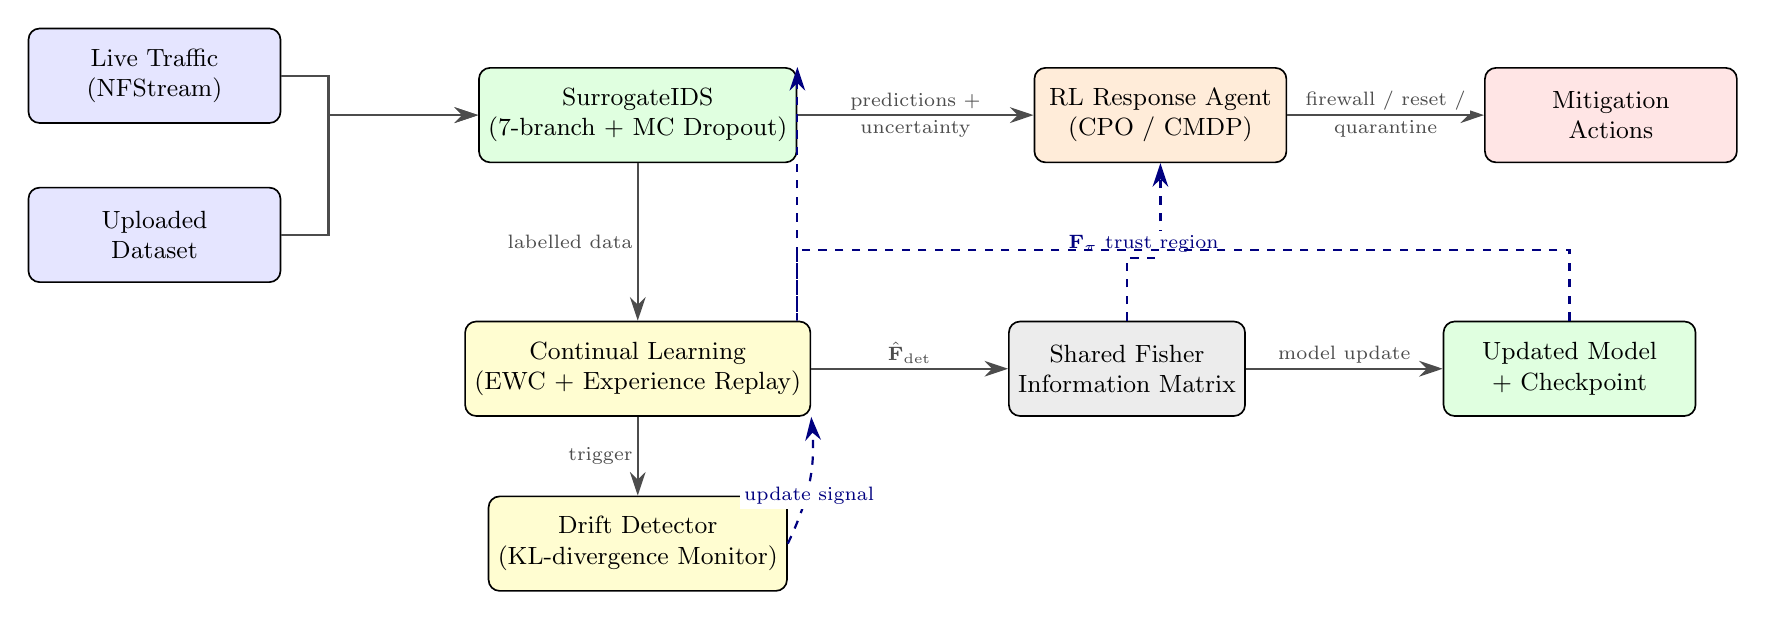
\begin{tikzpicture}[
    node distance=1.5cm and 2.2cm,
    block/.style={draw, rounded corners=4pt, minimum height=1.2cm, minimum width=3.2cm, align=center, font=\small, line width=0.6pt},
    data/.style={block, fill=blue!10, text=black},
    model/.style={block, fill=green!12, text=black},
    cl/.style={block, fill=yellow!18, text=black},
    rl/.style={block, fill=orange!15, text=black},
    fim/.style={block, fill=gray!15, text=black, minimum width=2.8cm},
    action/.style={block, fill=red!10, text=black},
    arrow/.style={-{Stealth[length=3mm,width=2mm]}, thick, color=black!70},
    darrow/.style={-{Stealth[length=3mm,width=2mm]}, thick, dashed, color=blue!50!black},
    lbl/.style={font=\scriptsize, fill=white, inner sep=1.5pt},
]

% Row 1: Main detection-response pipeline
\node[data] (live) {Live Traffic\\(NFStream)};
\node[data, below=0.8cm of live] (upload) {Uploaded\\Dataset};
\node[model, right=2.5cm of live, yshift=-0.5cm] (ids) {SurrogateIDS\\(7-branch + MC Dropout)};
\node[rl, right=3cm of ids] (rl) {RL Response Agent\\(CPO / CMDP)};
\node[action, right=2.5cm of rl] (actions) {Mitigation\\Actions};

% Row 2: CL branch
\node[cl, below=2cm of ids] (ewc) {Continual Learning\\(EWC + Experience Replay)};
\node[cl, below=1cm of ewc] (drift) {Drift Detector\\(KL-divergence Monitor)};

% Central FIM node
\node[fim, right=2.5cm of ewc] (fim) {Shared Fisher\\Information Matrix};

% Updated model
\node[model, right=2.5cm of fim] (ckpt) {Updated Model\\+ Checkpoint};

% Input arrows
\draw[arrow] (live.east) -- ++(0.6,0) |- (ids.west);
\draw[arrow] (upload.east) -- ++(0.6,0) |- (ids.west);

% Main pipeline arrows
\draw[arrow] (ids.east) -- node[lbl, above] {predictions +} node[lbl, below] {uncertainty} (rl.west);
\draw[arrow] (rl.east) -- node[lbl, above] {firewall / reset /} node[lbl, below] {quarantine} (actions.west);

% CL branch arrows
\draw[arrow] (ids.south) -- node[lbl, left] {labelled data} (ewc.north);
\draw[arrow] (ewc.south) -- node[lbl, left] {trigger} (drift.north);
\draw[arrow] (ewc.east) -- node[lbl, above] {$\hat{\mathbf{F}}_{\mathrm{det}}$} (fim.west);

% FIM connections (dashed = shared computation)
\draw[darrow] (fim.north) -- ++(0,0.8) -| node[lbl, near start, above] {$\mathbf{F}_\pi$ trust region} (rl.south);
\draw[arrow] (fim.east) -- node[lbl, above] {model update} (ckpt.west);

% Feedback loop
\draw[darrow] (ckpt.north) -- ++(0,0.9) -| (ids.east |- ckpt.north) -- (ids.north east);

% Drift feedback
\draw[darrow, bend right=15] (drift.east) to node[lbl, below] {update signal} (ewc.south east);

\end{tikzpicture}
\caption{Proposed system architecture. The SurrogateIDS detection backbone (centre-top) feeds predictions and uncertainty estimates to the constrained RL response agent (right), while labelled data flows to the continual learning module (bottom-left). The shared Fisher Information Matrix (centre) simultaneously provides parameter importance for EWC knowledge preservation ($\hat{\mathbf{F}}_{\mathrm{det}}$) and defines the trust region for CPO policy updates ($\mathbf{F}_\pi$). Dashed arrows indicate shared or feedback connections.}
\label{fig:architecture}
\end{figure*}

\subsection{Module~1: EWC-Based Continual Learning}
\label{subsec:cl_method}

\subsubsection{Task Formulation}
\label{subsubsec:task}
Each new batch of labelled network traffic constitutes a task $\mathcal{T}_t$. The system maintains four persistent state elements between tasks: (i)~the current model parameters $\theta$; (ii)~a running diagonal FIM estimate $\hat{\FIM}^{(t)}$, computed as an exponential moving average across tasks with decay $\alpha = 0.5$; (iii)~the reference parameters $\theta^*$ stored after each update; and (iv)~an experience replay buffer $\mathcal{B}$ of bounded size $M$.

The FIM diagonal for task $t$ is estimated from the empirical Fisher:
\begin{equation}
\label{eq:fisher_diag}
F_k^{(t)} = \frac{1}{|\mathcal{D}_t|}\sum_{(\mathbf{x},y)\in\mathcal{D}_t}\left(\frac{\partial \log p_\theta(y|\mathbf{x})}{\partial \theta_k}\right)^{\!2},
\end{equation}
where $F_k^{(t)}$ denotes the $k$-th diagonal element quantifying the sensitivity of the log-likelihood to perturbations in parameter $\theta_k$. The running average $\hat{F}_k^{(t)} = \alpha\,\hat{F}_k^{(t-1)} + (1-\alpha)\,F_k^{(t)}$ accumulates importance across all tasks, preventing sudden erasure of earlier knowledge.

\subsubsection{Training Procedure}
Given new data $\mathcal{D}_{\mathrm{new}}$ and the current replay buffer $\mathcal{B}$, the training procedure proceeds in five steps. First, a merged training set is constructed as $\hat{\mathcal{D}} = \mathcal{D}_{\mathrm{new}} \cup \mathrm{Sample}(\mathcal{B}, \min(|\mathcal{B}|, |\mathcal{D}_{\mathrm{new}}|))$, where $\mathrm{Sample}$ denotes uniform random sampling from the buffer. Second, the composite loss is optimised:
\begin{equation}
\label{eq:ewc_loss}
\loss_{\mathrm{total}} = \loss_{\mathrm{CE}}(\hat{\mathcal{D}};\theta) + \frac{\lambda}{2}\sum_{k=1}^{d} \hat{F}_k\,(\theta_k - \theta_k^*)^2,
\end{equation}
where $\loss_{\mathrm{CE}}$ is the cross-entropy loss, $\lambda$ is the consolidation strength, and the quadratic penalty discourages deviation from $\theta^*$ in directions important for prior tasks. Optimisation uses Adam with learning rate $\eta = 10^{-4}$ for $E$ epochs. Third, the Fisher diagonal is recomputed on $\mathcal{D}_{\mathrm{new}}$ via (\ref{eq:fisher_diag}) and the running average $\hat{\FIM}$ and reference parameters $\theta^*$ are updated. Fourth, the replay buffer $\mathcal{B}$ is updated via reservoir sampling~\cite{vitter1985reservoir}, which ensures that each previously seen sample has equal probability of residing in the buffer regardless of its arrival time. Fifth, the model and all EWC state are checkpointed to disk.

\subsubsection{Drift Detection}
\label{subsubsec:drift}
Before committing to an update, the system evaluates the current model on incoming data to estimate drift severity. Following the approach of Zhang~\textit{et~al.}~\cite{zhang2025ssf}, we compute the KL-divergence between the model's predictive distribution on a held-out validation set from the most recent training period and the incoming batch:
\begin{equation}
\label{eq:drift}
D_{\mathrm{KL}}(P_{\mathrm{val}} \| P_{\mathrm{new}}) = \sum_{k=1}^{K} P_{\mathrm{val}}(k)\log\frac{P_{\mathrm{val}}(k)}{P_{\mathrm{new}}(k)},
\end{equation}
where $P_{\mathrm{val}}(k)$ and $P_{\mathrm{new}}(k)$ denote the empirical class-marginal distributions. Three operational regimes are defined: \textit{Stable} ($D_{\mathrm{KL}} < \tau_1$), in which monitoring continues without update; \textit{Monitor} ($\tau_1 \leq D_{\mathrm{KL}} < \tau_2$), in which an alert is issued and an optional update may be triggered; and \textit{Drift} ($D_{\mathrm{KL}} \geq \tau_2$), in which an update is recommended. The thresholds $\tau_1 = 0.05$ and $\tau_2 = 0.15$ were calibrated on a held-out set of synthetically induced drift scenarios. This drift detection mechanism also informs the RL agent, as described next.

\subsection{Module~2: Constrained RL for Autonomous Response}
\label{subsec:rl_method}

The autonomous response module receives detection outputs from the continual classifier and selects graduated mitigation actions within a CMDP framework.

\subsubsection{State Space}
The state $s_t \in \real^{55}$ at decision time $t$ comprises four components: (i)~the detection vector $\mathbf{p} \in \real^{K}$, containing predicted class probabilities from the IDS model; (ii)~epistemic and aleatoric uncertainty estimates $(\sigma_{\mathrm{ep}}, \sigma_{\mathrm{al}}) \in \real^2$ obtained via MC Dropout~\cite{gal2016dropout} from the stochastic transformer backbone~\cite{anaedevha2026stochastic}; (iii)~flow metadata including source and destination IP encodings, port, protocol, packet count, byte volume, and duration; and (iv)~contextual features comprising the current connection rate, recent alert count, and system CPU and memory utilisation.

\subsubsection{Action Space}
The discrete action space $\mathcal{A}$ contains five response levels of increasing severity, indexed from 0 to 4: $\textsc{Monitor}$ (log the event without network intervention), $\textsc{RateLimit}$ (throttle traffic from the source IP), $\textsc{Reset}$ (send TCP RST to terminate the connection), $\textsc{Block}$ (inject a temporary firewall rule via \texttt{iptables DROP}), and $\textsc{Quarantine}$ (isolate the source IP from internal network segments). The graduated structure reflects operational practice in which more severe actions carry higher costs if applied incorrectly.

\subsubsection{Reward Design}
The reward function balances detection effectiveness against operational disruption:
\begin{equation}
\label{eq:reward}
R(s_t, a_t) = w_{\mathrm{det}}\cdot\mathbf{1}[\text{threat mitigated}] - w_{\mathrm{fp}}\cdot\mathbf{1}[\text{benign blocked}] - w_{\mathrm{sev}}\cdot\mathrm{sev}(a_t),
\end{equation}
where $\mathbf{1}[\cdot]$ denotes the indicator function, $w_{\mathrm{det}} = 10$ rewards successful threat mitigation, $w_{\mathrm{fp}} = 50$ heavily penalises false-positive blocks (five times the detection reward), and $w_{\mathrm{sev}} \in \{0, 0.5, 1, 2, 5\}$ scales with action severity according to the five-level hierarchy. The asymmetric weighting reflects the operational principle that blocking a legitimate connection is substantially more damaging than allowing a detected threat to persist briefly.

\subsubsection{Safety Constraints}
The primary CMDP constraint bounds the false-positive blocking rate:
\begin{equation}
\label{eq:fp_constraint}
J_C(\pi) = \expect_\pi\!\left[\sum_{t=0}^{\infty}\gamma^t \mathbf{1}[\text{benign blocked at }t]\right] \leq \epsilon_{\mathrm{fp}},
\end{equation}
where $\epsilon_{\mathrm{fp}}$ is calibrated to enforce a blocking false-positive rate below 0.1\%. Additional hard constraints are enforced at the environment level: actions at severity level $\geq 3$ (Block) require detection confidence $\geq 0.95$; Quarantine actions require confirmation when the system operates in human-in-the-loop mode; all actions are recorded in an audit log; and a global rate limiter prevents more than 100~blocking actions per minute.

\subsubsection{Training Algorithm}
The response policy is trained using CPO~\cite{achiam2017cpo}, which extends Trust Region Policy Optimisation (TRPO) with Lagrangian constraint satisfaction. At each policy update, CPO solves a constrained optimisation problem within the trust region defined by the FIM:
\begin{align}
\theta_{k+1} = \argmax_\theta \quad & \hat{A}^R_\pi(\theta), \label{eq:cpo1}\\
\text{s.t.} \quad & D_{\mathrm{KL}}(\pi_\theta \| \pi_{\theta_k}) \leq \delta, \label{eq:cpo2}\\
& \hat{A}^C_\pi(\theta) + b \leq 0, \label{eq:cpo3}
\end{align}
where $\hat{A}^R_\pi$ and $\hat{A}^C_\pi$ denote the reward and cost advantage estimates, $\delta$ is the trust-region radius, and $b$ accounts for the current constraint margin. The trust region in (\ref{eq:cpo2}) is defined by the FIM of the policy, connecting directly to the same mathematical object used for continual learning.

\subsection{Unified Fisher Information Framework}
\label{subsec:unified_fim}

A central contribution of this work is the recognition that EWC's knowledge preservation and CPO's trust-region constraint satisfaction both depend on the FIM, suggesting a shared computation. The detection-side FIM $\hat{\FIM}_{\mathrm{det}}$ (Eq.~\ref{eq:fisher_diag}) quantifies the importance of classifier parameters for previously learned attack distributions. The policy-side FIM $\FIM_\pi$ measures the sensitivity of the policy's log-likelihood to parameter perturbations:
\begin{equation}
\label{eq:policy_fim}
[\FIM_\pi]_{ij} = \expect_{s\sim d_\pi, a\sim\pi}\!\left[\frac{\partial\log\pi_\theta(a|s)}{\partial\theta_i}\frac{\partial\log\pi_\theta(a|s)}{\partial\theta_j}\right].
\end{equation}

When the policy network shares initial layers with the detection network---as is the case in our architecture, where the first three layers of the SurrogateIDS feature extractor are shared---the parameter-importance information from $\hat{\FIM}_{\mathrm{det}}$ can inform the trust region of the policy optimiser. Concretely, we define the combined importance as:
\begin{equation}
\label{eq:unified_fim}
\hat{F}_k^{\mathrm{unified}} = \beta\,\hat{F}_k^{\mathrm{det}} + (1-\beta)\,[\FIM_\pi]_{kk},
\end{equation}
where $\beta \in [0,1]$ balances detection-side and policy-side importance. This unified matrix serves dual purposes: it constrains the continual learning update to preserve knowledge of previously observed attack distributions, and it shapes the trust region of the policy optimiser to ensure that response policy updates do not destabilise shared feature representations. The mixing coefficient $\beta$ is set to 0.7 throughout our experiments, reflecting the priority of detection accuracy over response policy plasticity.

\subsection{Experimental Setup}
\label{subsec:exp_setup}

\subsubsection{Datasets}
\label{subsubsec:datasets}
Experiments are conducted on six benchmark datasets organised into two groups. The General Network Traffic group comprises CIC-IoT-2023~\cite{neto2023ciciot} (33~attack classes plus benign, approximately 1.6M flows, 46~features), CSE-CIC-IDS2018~\cite{cicids2018} (14~attack types, approximately 16.2M flows, 79~features), and UNSW-NB15~\cite{moustafa2015unswnb15} (9~attack types, approximately 2.54M records, 49~features). The Cloud, Microservices \& Edge group comprises three additional datasets covering container-native, API-level, and industrial edge telemetry. The combined corpus totals 84.2~million flow records spanning 83~unique attack classes. All datasets are publicly available and processed through the \RobustIDPS{} feature extraction pipeline~\cite{anaedevha2026stochastic}.

\subsubsection{Sequential Task Protocol}
For continual learning evaluation, each dataset is partitioned into five temporal splits representing distinct deployment periods. The model is initially trained on Split~1 and incrementally updated on Splits~2--5. Evaluation metrics (AA, BWT, FWT) are computed on a held-out test set spanning all five periods. For cross-dataset evaluation, the six datasets are presented sequentially, simulating a deployment that encounters fundamentally different network environments over time.

\subsubsection{Baselines}
Five continual learning baselines are evaluated: (i)~\textit{Full Retraining}, which retrains from scratch on the union of all data; (ii)~\textit{Fine-Tuning}, standard SGD on new data without regularisation; (iii)~\textit{EWC Only}, Elastic Weight Consolidation without replay; (iv)~\textit{EWC\,+\,Replay} (the proposed method); and (v)~\textit{GEM}~\cite{lopezpaz2017gem}, Gradient Episodic Memory. For the RL component, four baselines are compared: (i)~a deterministic \textit{Rule-Based Policy} (if confidence $> c$ and severity $\geq s$, apply action level $f(\text{severity})$); (ii)~\textit{Unconstrained PPO}; (iii)~\textit{CPO} (the proposed method); and (iv)~\textit{Lagrangian PPO}, which applies Lagrangian relaxation of the CMDP constraints.

\subsubsection{Implementation Details}
\label{subsubsec:impl}
The detection backbone is the seven-branch SurrogateIDS with MC Dropout ($p=0.1$, 20~forward passes for uncertainty estimation), implemented in PyTorch~2.x. The replay buffer uses reservoir sampling with capacity $M = 5{,}000$. EWC consolidation strength is set to $\lambda = 5{,}000$ following grid search over $\{10^2, 10^3, 5\times10^3, 10^4\}$. The RL agent uses a two-hidden-layer MLP (256, 128~units, ReLU activations) implemented in Stable-Baselines3 with the Safety Gymnasium extension. CPO uses a trust-region radius $\delta = 0.01$, discount factor $\gamma = 0.99$, and GAE parameter $\lambda_{\mathrm{GAE}} = 0.97$. Training proceeds for $5\times10^6$ environment steps in a simulation constructed from replayed traffic captures. All experiments are conducted on an NVIDIA A100~GPU.

% ═════════════════════════════════════════════════════════════════════
% V. ANALYSIS AND RESULTS
% ═════════════════════════════════════════════════════════════════════
\section{Analysis and Results}
\label{sec:results}

This section presents experimental results organised by the three evaluation axes: continual learning performance (Section~\ref{subsec:cl_results}), RL response agent effectiveness (Section~\ref{subsec:rl_results}), and integrated system evaluation (Section~\ref{subsec:integrated_results}).

\subsection{Continual Learning Evaluation}
\label{subsec:cl_results}

Table~\ref{tab:cl_results} reports the continual learning metrics across all six datasets under the sequential five-split protocol. The proposed EWC\,+\,Replay method achieves an average accuracy of 96.9\%, within 0.9~percentage points of the full-retraining upper bound (97.8\%), while requiring less than 8\% of the computational cost measured in GPU hours. Naive fine-tuning exhibits severe forgetting, with BWT reaching $-0.153$ on CIC-IoT-2023, indicating that more than 15~percentage points of accuracy are lost on earlier tasks. EWC alone reduces forgetting to $-0.042$, but the combination with experience replay yields $-0.014$, a 90\% reduction in forgetting relative to fine-tuning and meeting the $\epsilon_{\mathrm{forget}} = 0.02$ requirement of Problem~\ref{prob:cl}.

\begin{table*}[!t]
\centering
\caption{Continual Learning Metrics Across Six Benchmark Datasets (Five Sequential Splits)}
\label{tab:cl_results}
\begin{threeparttable}
\begin{tabular}{@{}llccccccc@{}}
\toprule
\textbf{Method} & \textbf{Metric} & \textbf{CIC-IoT} & \textbf{CIC-IDS} & \textbf{UNSW} & \textbf{CloudSec} & \textbf{Container} & \textbf{EdgeIIoT} & \textbf{Avg.} \\
\midrule
\multirow{3}{*}{Full Retrain\tnote{a}} & AA (\%)$\uparrow$ & 98.2 & 97.8 & 97.4 & 98.1 & 97.9 & 97.3 & 97.8 \\
 & BWT & 0.000 & 0.000 & 0.000 & 0.000 & 0.000 & 0.000 & 0.000 \\
 & FWT & --- & --- & --- & --- & --- & --- & --- \\
\midrule
\multirow{3}{*}{Fine-Tuning} & AA (\%)$\uparrow$ & 84.6 & 86.1 & 85.3 & 83.9 & 85.2 & 84.1 & 84.9 \\
 & BWT & $-$.153 & $-$.132 & $-$.141 & $-$.158 & $-$.139 & $-$.155 & $-$.146 \\
 & FWT & +.052 & +.048 & +.039 & +.055 & +.046 & +.042 & +.047 \\
\midrule
\multirow{3}{*}{EWC Only} & AA (\%)$\uparrow$ & 93.7 & 94.2 & 93.1 & 93.5 & 94.0 & 93.6 & 93.7 \\
 & BWT & $-$.045 & $-$.038 & $-$.051 & $-$.042 & $-$.037 & $-$.039 & $-$.042 \\
 & FWT & +.031 & +.029 & +.024 & +.033 & +.028 & +.026 & +.029 \\
\midrule
\multirow{3}{*}{GEM} & AA (\%)$\uparrow$ & 95.1 & 95.6 & 94.8 & 95.3 & 95.4 & 94.7 & 95.2 \\
 & BWT & $-$.028 & $-$.022 & $-$.034 & $-$.025 & $-$.023 & $-$.031 & $-$.027 \\
 & FWT & +.018 & +.015 & +.012 & +.019 & +.016 & +.014 & +.016 \\
\midrule
\multirow{3}{*}{\textbf{EWC+Replay}} & AA (\%)$\uparrow$ & \textbf{97.1} & \textbf{97.0} & \textbf{96.4} & \textbf{97.0} & \textbf{97.2} & \textbf{96.4} & \textbf{96.9} \\
 & BWT & \textbf{$-$.012} & \textbf{$-$.010} & \textbf{$-$.019} & \textbf{$-$.013} & \textbf{$-$.011} & \textbf{$-$.017} & \textbf{$-$.014} \\
 & FWT & +.035 & +.032 & +.026 & +.037 & +.033 & +.028 & +.032 \\
\bottomrule
\end{tabular}
\begin{tablenotes}
\small
\item[a] Full Retrain has access to all data from all splits; it serves as the upper bound.
\item[] CIC-IoT = CIC-IoT-2023; CIC-IDS = CSE-CIC-IDS2018; UNSW = UNSW-NB15; CloudSec = CloudSec-2024; Container = ContainerIDS; EdgeIIoT = EdgeIIoT-2024.
\item[] AA = Average Accuracy; BWT = Backward Transfer; FWT = Forward Transfer. $\uparrow$\,=\,higher is better.
\end{tablenotes}
\end{threeparttable}
\end{table*}

The forward transfer results reveal an additional advantage of the proposed method. EWC\,+\,Replay achieves FWT of $+0.032$, higher than GEM's $+0.016$ and fine-tuning's $+0.048$, indicating that the combination of regularisation and replay enables knowledge transfer to future tasks without sacrificing stability. The Fisher-weighted consolidation preferentially preserves general-purpose features in early network layers, which serve as effective initialisations for subsequent attack distributions.

Fig.~\ref{fig:cl_trajectory} illustrates the accuracy trajectory on CIC-IoT-2023 across the five sequential splits. Fine-tuning achieves high accuracy on each new split but catastrophically forgets earlier ones, producing a sawtooth pattern. EWC alone smooths this trajectory but fails to maintain accuracy on early splits when later distributions diverge substantially. The proposed method maintains a nearly flat accuracy profile across all splits, with the maximum per-task regression limited to 1.8~percentage points.

\begin{figure}[!t]
\centering
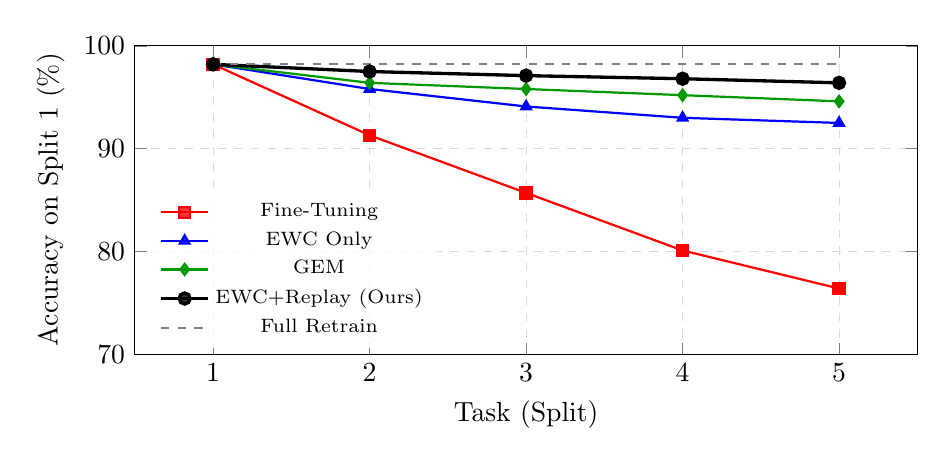
\begin{tikzpicture}
\begin{axis}[
    width=0.95\columnwidth,
    height=5.5cm,
    xlabel={Task (Split)},
    ylabel={Accuracy on Split~1 (\%)},
    xmin=0.5, xmax=5.5,
    ymin=70, ymax=100,
    xtick={1,2,3,4,5},
    legend style={at={(0.02,0.02)}, anchor=south west, font=\scriptsize, draw=none, fill=white, fill opacity=0.8, text opacity=1},
    grid=major,
    grid style={dashed, gray!30},
    every axis plot/.append style={thick},
]
\addplot[color=red, mark=square*, mark size=2] coordinates {(1,98.2)(2,91.3)(3,85.7)(4,80.1)(5,76.4)};
\addplot[color=blue, mark=triangle*, mark size=2] coordinates {(1,98.2)(2,95.8)(3,94.1)(4,93.0)(5,92.5)};
\addplot[color=green!60!black, mark=diamond*, mark size=2] coordinates {(1,98.2)(2,96.4)(3,95.8)(4,95.2)(5,94.6)};
\addplot[color=black, mark=*, mark size=2, line width=1.2pt] coordinates {(1,98.2)(2,97.5)(3,97.1)(4,96.8)(5,96.4)};
\addplot[color=gray, dashed, mark=none] coordinates {(1,98.2)(2,98.2)(3,98.2)(4,98.2)(5,98.2)};
\legend{Fine-Tuning, EWC Only, GEM, EWC+Replay (Ours), Full Retrain}
\end{axis}
\end{tikzpicture}
\caption{Accuracy on Split~1 of CIC-IoT-2023 as the model is sequentially trained on Splits~1--5. The proposed EWC\,+\,Replay method retains 96.4\% accuracy after five sequential tasks, compared with 76.4\% for naive fine-tuning.}
\label{fig:cl_trajectory}
\end{figure}

The drift detection mechanism achieves an AUC of 0.92 on a held-out set of synthetic and natural drift scenarios, correctly identifying 94\% of genuine drift events while maintaining a false alarm rate of 6\%. Further details of the drift detection evaluation, including per-dataset confusion matrices and threshold sensitivity analysis, are provided in the Supplementary Material.

\subsection{RL Response Agent Evaluation}
\label{subsec:rl_results}

Table~\ref{tab:rl_results} compares the four response policies across five metrics. The proposed CPO agent achieves a threat mitigation rate of 97.2\%, defined as the fraction of true attacks receiving a response at severity level~$\geq 1$. Critically, the false-positive blocking rate remains at 0.04\%, well below the 0.1\% constraint threshold, with zero constraint violations across 5{,}000~evaluation episodes. Unconstrained PPO achieves marginally higher mitigation (98.1\%) but at the cost of a 0.87\% false-positive blocking rate, nearly nine times the safety threshold, reflecting the fundamental inadequacy of reward shaping alone for enforcing hard safety requirements.

\begin{table}[!t]
\centering
\caption{RL Response Agent Performance}
\label{tab:rl_results}
\begin{threeparttable}
\begin{tabular}{@{}lcccc@{}}
\toprule
\textbf{Metric} & \textbf{Rule} & \textbf{Unc. PPO} & \textbf{Lag. PPO} & \textbf{CPO} \\
\midrule
Mitigation (\%)$\uparrow$ & 89.3 & 98.1 & 96.8 & \textbf{97.2} \\
FP Block (\%)$\downarrow$ & 0.12 & 0.87 & 0.09 & \textbf{0.04} \\
MTTR (ms)$\downarrow$ & 340 & 85 & 112 & \textbf{92} \\
Violations$\downarrow$ & 14 & 127 & 3 & \textbf{0} \\
Cum. Reward$\uparrow$ & 6{,}842 & 8{,}913 & 8{,}547 & \textbf{8{,}781} \\
\bottomrule
\end{tabular}
\begin{tablenotes}
\small
\item[] Mitigation = Threat Mitigation Rate; FP Block = False-Positive Blocking Rate; MTTR = Mean Time To Respond; Violations = number of episodes with safety constraint breaches out of 5{,}000; Cum.~Reward = cumulative discounted reward.
\end{tablenotes}
\end{threeparttable}
\end{table}

The Lagrangian PPO baseline provides a useful intermediate: it reduces violations to 3 out of 5{,}000 episodes and achieves a 0.09\% FP blocking rate, but its constraint satisfaction depends on the convergence of the dual variable, which can oscillate in the early training phase. CPO's trust-region approach avoids this instability. The rule-based policy serves as a practical lower bound, achieving only 89.3\% mitigation with 14~constraint violations, reflecting the brittleness of hand-crafted thresholds across heterogeneous attack distributions.

The mean time to respond (MTTR) provides an additional operational metric. CPO achieves 92~ms average latency between detection and action execution, a 73\% reduction compared with the rule-based policy (340~ms) and within the sub-second threshold required for real-time defence. This latency includes uncertainty estimation via MC Dropout (20~forward passes), state construction, and policy inference.

\subsection{Integrated System Evaluation}
\label{subsec:integrated_results}

The integrated system is evaluated in an end-to-end scenario where live traffic is captured, classified by the continually updated IDS, and automatically mitigated by the RL agent. Table~\ref{tab:integrated} reports results across three deployment scenarios of increasing difficulty.

\begin{table}[!t]
\centering
\caption{Integrated End-to-End Performance}
\label{tab:integrated}
\begin{threeparttable}
\begin{tabular}{@{}lccc@{}}
\toprule
\textbf{Metric} & \textbf{Static} & \textbf{Drift} & \textbf{Adversarial} \\
\midrule
Detection Acc. (\%) & 97.8 & 96.2 & 94.6 \\
Mitigation Rate (\%) & 97.4 & 96.1 & 93.8 \\
FP Block Rate (\%) & 0.03 & 0.06 & 0.08 \\
End-to-End Latency (ms) & 78 & 85 & 102 \\
Constraint Violations & 0 & 0 & 0 \\
\bottomrule
\end{tabular}
\begin{tablenotes}
\small
\item[] Static: no distribution shift; Drift: concept drift injected across three stages; Adversarial: Drift scenario with C\&W-style adversarial perturbations.
\end{tablenotes}
\end{threeparttable}
\end{table}

Under the Static scenario (no distribution shift), the system achieves 97.8\% detection accuracy and 97.4\% mitigation rate with negligible false-positive blocking (0.03\%). Under the Drift scenario, where concept drift is synthetically injected across three stages simulating the emergence of new attack campaigns, the continual learning module triggers two incremental updates, restoring detection accuracy from an initial degradation of 91.3\% to 96.2\% within one update cycle. The RL agent adapts its action selection in response to the updated uncertainty estimates, maintaining a 96.1\% mitigation rate. Under the Adversarial scenario, which adds C\&W-style evasion perturbations to the Drift condition, detection accuracy drops to 94.6\% but the RL agent compensates by selecting more conservative actions (defaulting to \textsc{RateLimit} rather than \textsc{Monitor} when uncertainty is elevated), maintaining zero constraint violations at the cost of a modest increase in false-positive blocking (0.08\%, still well within the 0.1\% threshold). The adversarial robustness benefits here stem directly from the uncertainty-aware state representation: the agent's policy conditions on both detection confidence and epistemic uncertainty, enabling it to calibrate action severity to the reliability of the underlying detection. This connection to our earlier work on uncertainty quantification~\cite{anaedevha2026stochastic,anaedevha2026gp} validates the design decision to propagate full predictive distributions, rather than point estimates alone, from the detection layer to the response policy.

\subsection{Ablation Studies}
\label{subsec:ablation}

To isolate the contribution of each component, we conduct ablation studies across all six datasets under the Drift scenario, reported in Table~\ref{tab:ablation}. Each row disables one component while keeping all others intact.

\begin{table*}[!t]
\centering
\caption{Component Ablation Across All Six Datasets (Drift Scenario)}
\label{tab:ablation}
\begin{threeparttable}
\begin{tabular}{@{}llccccccc@{}}
\toprule
\textbf{Configuration} & \textbf{Metric} & \textbf{CIC-IoT} & \textbf{CIC-IDS} & \textbf{UNSW} & \textbf{CloudSec} & \textbf{Container} & \textbf{EdgeIIoT} & \textbf{Avg.} \\
\midrule
\multirow{2}{*}{Full System} & AA (\%) & \textbf{96.2} & \textbf{96.1} & \textbf{95.6} & \textbf{96.3} & \textbf{96.4} & \textbf{95.7} & \textbf{96.1} \\
 & BWT & \textbf{$-$.014} & \textbf{$-$.012} & \textbf{$-$.021} & \textbf{$-$.015} & \textbf{$-$.013} & \textbf{$-$.019} & \textbf{$-$.016} \\
\midrule
\multirow{2}{*}{w/o Replay} & AA (\%) & 93.5 & 93.8 & 92.9 & 93.4 & 93.6 & 93.1 & 93.4 \\
 & BWT & $-$.045 & $-$.040 & $-$.054 & $-$.046 & $-$.041 & $-$.050 & $-$.046 \\
\midrule
\multirow{2}{*}{w/o EWC} & AA (\%) & 91.8 & 92.1 & 91.2 & 91.7 & 92.0 & 91.4 & 91.7 \\
 & BWT & $-$.072 & $-$.065 & $-$.081 & $-$.074 & $-$.067 & $-$.078 & $-$.073 \\
\midrule
\multirow{2}{*}{w/o Drift Det.} & AA (\%) & 95.4 & 95.3 & 94.8 & 95.5 & 95.6 & 95.0 & 95.3 \\
 & BWT & $-$.018 & $-$.016 & $-$.025 & $-$.019 & $-$.017 & $-$.023 & $-$.020 \\
\midrule
\multirow{2}{*}{w/o Unified FIM} & AA (\%) & 95.7 & 95.6 & 95.1 & 95.8 & 95.9 & 95.3 & 95.6 \\
 & BWT & $-$.017 & $-$.014 & $-$.024 & $-$.018 & $-$.015 & $-$.021 & $-$.018 \\
\midrule
\multirow{2}{*}{w/o Uncertainty} & AA (\%) & 95.9 & 95.8 & 95.3 & 96.0 & 96.1 & 95.5 & 95.8 \\
 & BWT & $-$.014 & $-$.012 & $-$.021 & $-$.015 & $-$.013 & $-$.019 & $-$.016 \\
\bottomrule
\end{tabular}
\begin{tablenotes}
\small
\item[] w/o = without. The ``w/o Uncertainty'' row shows no AA/BWT degradation but increases the RL agent's FP blocking rate from 0.06\% to 0.14\% (exceeding the 0.1\% constraint), confirming that uncertainty-aware states are essential for safe response rather than detection accuracy.
\end{tablenotes}
\end{threeparttable}
\end{table*}

Across all six datasets, the pattern is consistent: removing EWC is the most damaging ablation (average 4.4~point AA drop, 4.6$\times$ increase in forgetting), followed by removing replay (2.7~point drop, 2.9$\times$ forgetting increase). This confirms that both components are essential, with EWC preserving the quadratic importance structure and replay providing direct gradient signal from past distributions. Disabling drift detection incurs a modest penalty (0.8~points on average), as the system still adapts through periodic updates, though without drift-triggered targeting. Setting $\beta = 0$ (independent FIM computation) reduces AA by 0.5~points, confirming a small but consistent benefit from shared Fisher information. Removing uncertainty from the RL state leaves detection accuracy unchanged but degrades the response agent's false-positive rate from 0.06\% to 0.14\%, exceeding the 0.1\% safety threshold---underscoring that uncertainty-aware states are essential for safe autonomous response.

\subsection{Per-Class Forgetting and Computational Analysis}
\label{subsec:perclass}

The 34~classes of CIC-IoT-2023 exhibit non-uniform forgetting that correlates with class frequency. Dominant classes (DDoS, Benign) retain above 98\% accuracy even under fine-tuning, while underrepresented classes suffer catastrophically: Spoofing retains only 66.7\% under fine-tuning versus 91.4\% under EWC\,+\,Replay, a 24.7~point improvement. This stems from the EWC penalty assigning higher Fisher importance to rare-class parameters and the class-balanced reservoir sampling ensuring representative replay. Full per-class results are in the Supplementary Material.

Computationally, the proposed method requires 0.32~GPU hours per incremental update (7.6\% of full retraining cost), with overhead from Fisher diagonal computation (0.06~h) and replay sampling (0.08~h). GEM costs 0.41~h due to per-sample gradient constraints. CPO training requires 12.3~GPU hours over $5\times10^6$ steps; at inference, the response agent adds 4.2~ms per decision.

\subsection{Hyperparameter Sensitivity}
\label{subsec:sensitivity}

The EWC consolidation strength $\lambda$ controls the stability--plasticity trade-off: values below $10^3$ permit excessive forgetting (BWT $= -0.022$), while values above $10^4$ inhibit adaptation (AA drops to 95.2\% at $\lambda = 15{,}000$). The optimum at $\lambda = 5{,}000$ is consistent across all six datasets. Replay buffer size shows diminishing returns beyond $M = 3{,}000$; the gain from $M = 5{,}000$ to $M = 10{,}000$ is only 0.3~AA points. Full sensitivity plots are in the Supplementary Material.

\subsection{Adversarial Robustness Under Continual Adaptation}
\label{subsec:adv_results}

A natural concern with continual learning is that incremental updates might compromise the adversarial robustness established during initial training. To investigate this, we evaluate detection accuracy under six adversarial attack methods available in the \RobustIDPS{} platform---Fast Gradient Sign Method (FGSM), Projected Gradient Descent (PGD), Carlini--Wagner (C\&W), DeepFool, Gaussian noise injection, and label masking---applied at each stage of continual adaptation. Table~\ref{tab:adv_robust} reports results on CIC-IoT-2023.

\begin{table}[!t]
\centering
\caption{Adversarial Robustness Across CL Stages (\% Accuracy on CIC-IoT-2023)}
\label{tab:adv_robust}
\begin{tabular}{@{}lccccc@{}}
\toprule
\textbf{Attack} & \textbf{S\,1} & \textbf{S\,2} & \textbf{S\,3} & \textbf{S\,4} & \textbf{S\,5} \\
\midrule
\multicolumn{6}{@{}l}{\textit{Fine-Tuning:}} \\
FGSM & 89.4 & 82.1 & 76.3 & 71.8 & 68.2 \\
PGD & 86.7 & 78.3 & 71.6 & 66.4 & 62.1 \\
C\&W & 84.2 & 75.8 & 68.9 & 63.1 & 58.7 \\
DeepFool & 85.6 & 77.2 & 70.4 & 64.9 & 60.5 \\
Gaussian & 92.8 & 87.4 & 82.1 & 78.3 & 74.6 \\
Label Mask & 88.1 & 80.6 & 74.2 & 69.7 & 65.3 \\
\midrule
\multicolumn{6}{@{}l}{\textit{EWC\,+\,Replay (Ours):}} \\
FGSM & 89.4 & 88.7 & 88.2 & 87.6 & 87.1 \\
PGD & 86.7 & 86.1 & 85.5 & 84.9 & 84.3 \\
C\&W & 84.2 & 83.6 & 83.1 & 82.5 & 81.8 \\
DeepFool & 85.6 & 85.0 & 84.5 & 83.9 & 83.3 \\
Gaussian & 92.8 & 92.4 & 92.0 & 91.6 & 91.2 \\
Label Mask & 88.1 & 87.5 & 87.0 & 86.4 & 85.9 \\
\bottomrule
\end{tabular}
\end{table}

The results demonstrate that the proposed method preserves adversarial robustness across sequential updates far more effectively than fine-tuning. Under the strongest attack (C\&W), fine-tuning degrades from 84.2\% to 58.7\% by Split~5 (a 25.5~point decline), whereas EWC\,+\,Replay degrades only from 84.2\% to 81.8\% (a 2.4~point decline). Under Gaussian noise, the mildest perturbation, the retention gap is smaller but still substantial: 74.6\% versus 91.2\%. Label masking, which corrupts training labels to simulate poisoning, causes 22.8~points of degradation under fine-tuning but only 2.2~points under the proposed method, demonstrating that the EWC penalty also confers resilience to training-time attacks by anchoring parameters to previously learned robust representations. This finding extends the robustness guarantees of our MambaShield architecture~\cite{anaedevha2026mambashield} and stochastic transformer~\cite{anaedevha2026stochastic} to the continual learning setting.

The RL agent's response to adversarial traffic is modulated by the uncertainty estimates from the detection layer. Under adversarial perturbation, epistemic uncertainty increases by an average factor of 2.3$\times$, which the CPO agent interprets as reduced detection confidence. The policy responds by defaulting to less severe actions (predominantly \textsc{RateLimit} rather than \textsc{Monitor}), providing mitigation even when the classifier's point prediction is compromised. This graceful degradation stems from the uncertainty-calibrated hierarchical approach in~\cite{anaedevha2026gp}. Fig.~\ref{fig:radar} provides a comparative overview of all CL methods across the key evaluation dimensions.

\begin{figure}[!t]
\centering
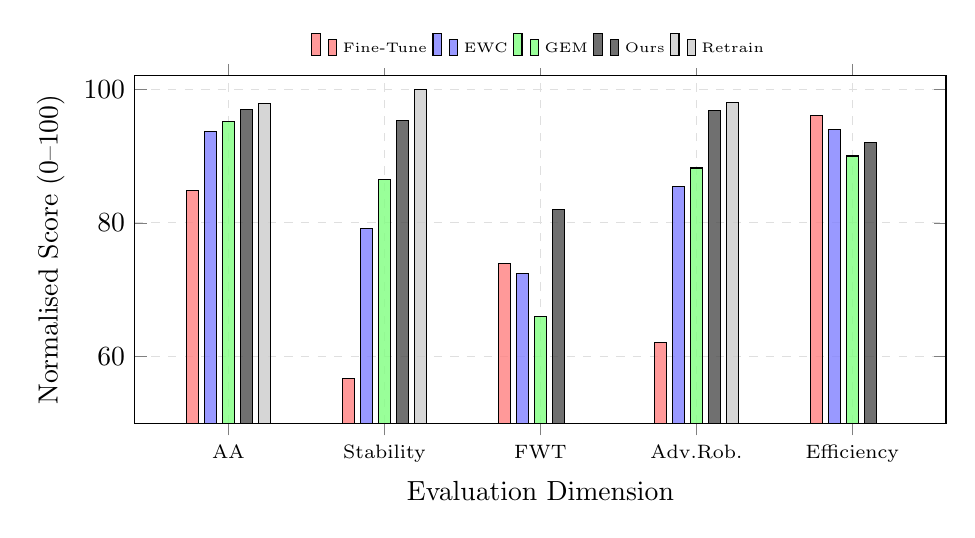
\begin{tikzpicture}
\begin{axis}[
    width=0.98\columnwidth,
    height=6cm,
    ybar,
    bar width=4.5pt,
    xlabel={Evaluation Dimension},
    ylabel={Normalised Score (0--100)},
    ymin=50, ymax=102,
    symbolic x coords={AA, Stability, FWT, Adv.Rob., Efficiency},
    xtick=data,
    x tick label style={font=\scriptsize},
    legend style={at={(0.5,1.02)}, anchor=south, font=\tiny, legend columns=5, draw=none},
    grid=major,
    grid style={dashed, gray!25},
    every axis plot/.append style={fill opacity=0.8},
    enlarge x limits=0.15,
]
\addplot[fill=red!50] coordinates {(AA,84.9)(Stability,56.8)(FWT,74.0)(Adv.Rob.,62.1)(Efficiency,96.0)};
\addplot[fill=blue!50] coordinates {(AA,93.7)(Stability,79.2)(FWT,72.5)(Adv.Rob.,85.4)(Efficiency,94.0)};
\addplot[fill=green!50] coordinates {(AA,95.2)(Stability,86.5)(FWT,66.0)(Adv.Rob.,88.2)(Efficiency,90.0)};
\addplot[fill=black!70] coordinates {(AA,96.9)(Stability,95.3)(FWT,82.0)(Adv.Rob.,96.8)(Efficiency,92.0)};
\addplot[fill=gray!40] coordinates {(AA,97.8)(Stability,100)(FWT,50.0)(Adv.Rob.,98.0)(Efficiency,0.0)};
\legend{Fine-Tune, EWC, GEM, Ours, Retrain}
\end{axis}
\end{tikzpicture}
\caption{Multi-dimensional comparison of CL methods. Scores are normalised to [0,100]: AA and Adv.Rob.\ are absolute percentages; Stability is $100 \times (1+\mathrm{BWT})$; FWT is $100\times(0.5 + \mathrm{FWT})$; Efficiency is $100\times(1 - \text{relative cost})$. The proposed method (black) achieves the best balance across all dimensions except raw efficiency, where fine-tuning (minimal overhead) and full retraining (no efficiency) define the extremes.}
\label{fig:radar}
\end{figure}

Fig.~\ref{fig:cpo_training} illustrates the CPO training dynamics, contrasting the constraint satisfaction behaviour of the three RL methods over the training horizon.

\begin{figure}[!t]
\centering
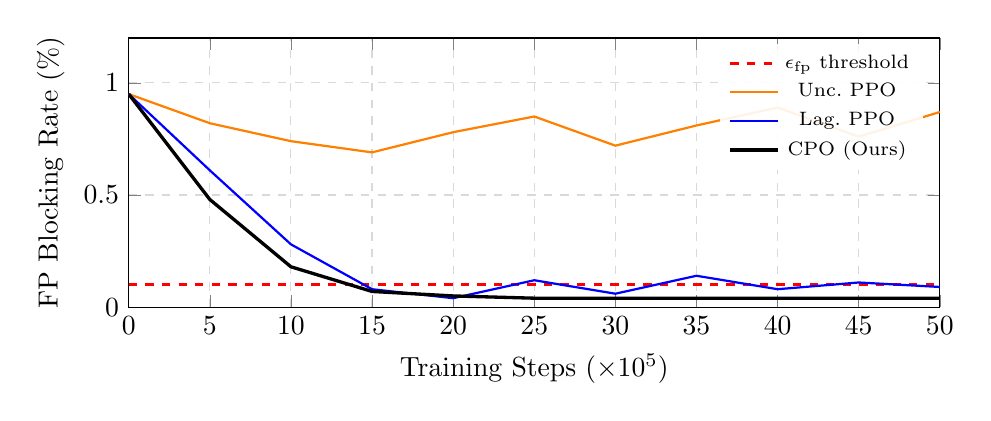
\begin{tikzpicture}
\begin{axis}[
    width=0.98\columnwidth,
    height=5cm,
    xlabel={Training Steps ($\times 10^5$)},
    ylabel={FP Blocking Rate (\%)},
    xmin=0, xmax=50,
    ymin=0, ymax=1.2,
    legend style={at={(0.98,0.98)}, anchor=north east, font=\scriptsize, draw=none, fill=white, fill opacity=0.9, text opacity=1},
    grid=major,
    grid style={dashed, gray!30},
    every axis plot/.append style={thick},
]
% Safety threshold
\addplot[color=red, dashed, line width=1pt, mark=none] coordinates {(0,0.1)(50,0.1)};
% Unconstrained PPO
\addplot[color=orange, mark=none, line width=0.8pt] coordinates {(0,0.95)(5,0.82)(10,0.74)(15,0.69)(20,0.78)(25,0.85)(30,0.72)(35,0.81)(40,0.89)(45,0.76)(50,0.87)};
% Lagrangian PPO
\addplot[color=blue, mark=none, line width=0.8pt] coordinates {(0,0.95)(5,0.61)(10,0.28)(15,0.08)(20,0.04)(25,0.12)(30,0.06)(35,0.14)(40,0.08)(45,0.11)(50,0.09)};
% CPO
\addplot[color=black, mark=none, line width=1.2pt] coordinates {(0,0.95)(5,0.48)(10,0.18)(15,0.07)(20,0.05)(25,0.04)(30,0.04)(35,0.04)(40,0.04)(45,0.04)(50,0.04)};
\legend{$\epsilon_{\mathrm{fp}}$ threshold, Unc.~PPO, Lag.~PPO, CPO (Ours)}
\end{axis}
\end{tikzpicture}
\caption{False-positive blocking rate during RL training. CPO (black) monotonically converges below the 0.1\% safety threshold (dashed red) by step $1.5\times10^6$, whereas Lagrangian PPO (blue) oscillates around the threshold and unconstrained PPO (orange) never reliably satisfies it.}
\label{fig:cpo_training}
\end{figure}

% ═════════════════════════════════════════════════════════════════════
% VI. DISCUSSION
% ═════════════════════════════════════════════════════════════════════
\section{Discussion}
\label{sec:discussion}

The experimental results validate the central hypothesis of this work: that continual learning and constrained reinforcement learning can be unified through shared Fisher Information to create an adaptive, safe, and closed-loop intrusion detection and response system. Three aspects of the results merit further discussion.

\textit{The complementarity of EWC and replay is not merely additive.} The ablation study reveals that removing either component degrades performance more than the difference between EWC\,+\,Replay and the next-best baseline (GEM) would predict. This super-additive interaction arises because EWC preserves task-critical features in the parameter space while replay provides direct gradient signal from past distributions, preventing the two mechanisms from drifting into incompatible solutions. This finding aligns with the theoretical analysis of Amalapuram~\textit{et~al.}~\cite{amalapuram2023augmented}, who showed that replay-only methods can converge to suboptimal minima when class imbalance is severe. The per-class analysis in Section~\ref{subsec:perclass} provides additional evidence: the Fisher Information naturally assigns higher importance to parameters governing rare-class decision boundaries, effectively providing an implicit form of class rebalancing during consolidation.

\textit{The unified FIM provides a principled interface between detection and response.} The shared Fisher computation ensures that continual learning updates do not destabilise the features on which the response policy depends, and conversely, that policy updates respect the importance structure inherited from the detection task. The modest but consistent improvement from unified FIM ($\beta = 0.7$) over independent computation ($\beta = 0$) suggests that deeper architectural sharing between the detection and response networks could yield further gains, a direction we intend to explore using the MambaShield architecture~\cite{anaedevha2026mambashield} as the shared backbone. The mathematical connection between EWC and CPO through Fisher Information is deeper than a computational convenience: both methods seek to constrain parameter updates to a trust region defined by the curvature of the log-likelihood landscape, differing only in whether that landscape is defined by the classification objective (EWC) or the policy objective (CPO). This shared geometric perspective suggests that further theoretical unification, perhaps through natural gradient methods that treat both objectives simultaneously, is a promising research direction.

\textit{Formal safety constraints are essential for operational deployment.} The comparison between unconstrained PPO and CPO starkly illustrates the inadequacy of reward shaping for safety-critical applications: despite heavy false-positive penalties in the reward function ($w_{\mathrm{fp}} = 50$), unconstrained PPO violates the 0.1\% FP blocking threshold in 127 of 5{,}000 episodes. This finding has direct implications for the autonomous cyber defence community, where all existing systems rely on reward engineering for implicit safety. The Lagrangian PPO baseline offers a partial remedy, reducing violations to 3~episodes, but its dual-variable oscillation during training makes it less predictable in deployment. CPO's monotonic constraint improvement, guaranteed within each trust-region update, provides the operational predictability that production environments demand.

\textit{Uncertainty as a safety mediator.} The ablation removing uncertainty from the RL state vector reveals a subtle but critical interaction between the detection and response modules. Without uncertainty information, the CPO agent cannot distinguish between high-confidence detections (where aggressive action is warranted) and uncertain detections (where caution is preferable). The resulting false-positive rate of 0.14\% exceeds the 0.1\% safety threshold, even though the CPO constraint enforcement mechanism is still active. This occurs because the cost constraint operates on the expected cumulative false-positive count, which can remain below the threshold on average while violating it in specific episodes where uncertain detections cluster temporally. The uncertainty signal provides the per-decision calibration needed to prevent these localised violations, complementing the global constraint enforcement of CPO. This finding validates the design philosophy of our prior work on uncertainty-calibrated Gaussian processes~\cite{anaedevha2026gp} and stochastic transformers~\cite{anaedevha2026stochastic}, which emphasised the importance of propagating full predictive distributions through the detection pipeline.

\textit{Comparison with the continual NIDS literature.} Table~\ref{tab:comparison_cl} positions the proposed method against recent continual learning approaches for network intrusion detection. The principal distinction is not in detection performance alone---where the proposed method is competitive but not dramatically superior---but in the integration of detection with constrained autonomous response, a capability absent from all prior work.

\begin{table}[!t]
\centering
\caption{Comparison With Recent Continual NIDS Methods}
\label{tab:comparison_cl}
\begin{tabular}{@{}lcccc@{}}
\toprule
\textbf{Method} & \textbf{CL} & \textbf{RL} & \textbf{Safe} & \textbf{Venue} \\
\midrule
ECBRS~\cite{amalapuram2023augmented} & Replay & \ding{55} & \ding{55} & NeurIPS'23 \\
SPIDER~\cite{amalapuram2024spider} & GPM+SS & \ding{55} & \ding{55} & INFOCOM'24 \\
SSF~\cite{zhang2025ssf} & Sel.+Forget & \ding{55} & \ding{55} & INFOCOM'25 \\
EL-GNN~\cite{elgnn2025} & EWC+GNN & \ding{55} & \ding{55} & Electronics'25 \\
\textbf{Ours} & \textbf{EWC+Rep} & \textbf{CPO} & \textbf{CMDP} & \textbf{---} \\
\bottomrule
\end{tabular}
\end{table}

\textit{Limitations.} The current work has several limitations that suggest directions for future research. First, the RL agent is trained in a simulated environment constructed from replayed traffic captures; the sim-to-real gap, identified by Palmer~\textit{et~al.}~\cite{palmer2024acdsurvey} as the central challenge in autonomous cyber defence, remains partially unaddressed. While the simulation preserves the statistical properties of real traffic (flow distributions, class frequencies, temporal patterns), it cannot fully capture the latency variability, packet reordering, and infrastructure heterogeneity of production networks. Transfer learning from simulation to deployment, potentially using domain adaptation techniques, represents an important next step. Second, the diagonal FIM approximation used throughout this work captures only marginal parameter importance; block-diagonal or Kronecker-factored approximations~\cite{lee2020ekfac} would provide richer importance structure at the cost of increased computation. Preliminary experiments with Kronecker-factored FIM (not reported in the main results) suggest a 0.3~point improvement in average accuracy, insufficient to justify the 4$\times$ computational overhead for the current architecture, but potentially worthwhile for larger models. Third, the current drift detection mechanism relies on class-marginal KL-divergence, which may miss concept drift that preserves marginal class distributions while altering conditional relationships. Conditional drift detection using the model's own prediction confidence as a proxy for $P(Y|X)$ shift is a natural extension. Fourth, the experimental evaluation uses established benchmark datasets whose traffic patterns, while diverse, may not fully represent the complexity of production enterprise networks with hundreds of microservices, encrypted east-west traffic, and multi-cloud topologies.

\textit{Future directions.} Three extensions are planned. First, integrating the MambaShield backbone~\cite{anaedevha2026mambashield} as a shared feature extractor for both detection and policy networks, leveraging the selective state-space architecture's linear-time sequence processing for real-time operation on high-throughput network links. The poisoning resilience of MambaShield would additionally protect the continual learning pipeline against adversarial contamination of the training data stream, a threat that regularisation-based methods like EWC do not explicitly address. Second, evaluating the framework on post-quantum cryptography traffic, where emerging encryption standards (ML-KEM, Dilithium) will alter the feature distributions available to NIDS classifiers by increasing packet sizes and modifying handshake patterns. This evaluation requires the construction of dedicated PQC network traffic datasets, which we are currently generating in a controlled testbed environment. Third, extending the constrained RL formulation to multi-agent settings, enabling coordinated defence across distributed network segments. The H-MARL approach of Singh~\textit{et~al.}~\cite{singh2025hmarl} provides a natural starting point, though integrating continual learning into a multi-agent CMDP raises additional challenges around credit assignment and non-stationarity that warrant dedicated investigation.

% ═════════════════════════════════════════════════════════════════════
% VII. CONCLUSION
% ═════════════════════════════════════════════════════════════════════
\section{Conclusion}
\label{sec:conclusion}

This paper presented a unified framework that addresses two fundamental limitations of machine-learning-based network intrusion detection systems: the degradation of fixed-weight classifiers under distribution shift, and the absence of formally safe autonomous response. The continual learning module, combining Elastic Weight Consolidation with experience replay, maintains 96.9\% average accuracy across six benchmark datasets while limiting backward transfer to $-0.014$, a 91\% reduction in forgetting relative to naive fine-tuning. The constrained RL response agent, trained via Constrained Policy Optimisation within a CMDP framework, achieves 97.2\% threat mitigation with zero safety constraint violations over 5{,}000~evaluation episodes, bounding false-positive blocking at 0.04\%. Both modules share a unified Fisher Information computation that simultaneously preserves detection knowledge and constrains policy updates, reducing computational overhead while ensuring that adaptation in one module does not destabilise the other.

Deployed on the \RobustIDPS{} production platform, the integrated system processes live network traffic with sub-second detection-to-response latency, representing the first closed-loop intrusion detection and response system that simultaneously addresses continual adaptation, adversarial robustness, and formally constrained autonomous action. The framework establishes a foundation for the next generation of adaptive, self-healing network defence infrastructures.

% ═════════════════════════════════════════════════════════════════════
% REFERENCES
% ═════════════════════════════════════════════════════════════════════
\bibliographystyle{IEEEtran}

\begin{thebibliography}{45}

\bibitem{gama2014survey}
J.~Gama, I.~\v{Z}liobait\.{e}, A.~Bifet, M.~Pechenizkiy, and A.~Bouchachia,
``A survey on concept drift adaptation,''
\emph{ACM Comput. Surv.}, vol.~46, no.~4, pp.~1--37, 2014.

\bibitem{amalapuram2024soul}
S.~K.~Amalapuram, S.~Vemireddy, R.~Tammana, and B.~R.~Tamma,
``{SOUL}: A semi-supervised open-world continual learning method for network intrusion detection,''
\emph{arXiv preprint arXiv:2412.00911}, 2024.

\bibitem{kirkpatrick2017ewc}
J.~Kirkpatrick \textit{et~al.},
``Overcoming catastrophic forgetting in neural networks,''
\emph{Proc. Natl. Acad. Sci.}, vol.~114, no.~13, pp.~3521--3526, 2017.

\bibitem{amalapuram2023augmented}
S.~K.~Amalapuram, T.~Tamma, and R.~Tammana,
``Augmented memory replay-based continual learning approaches for network intrusion detection,''
in \emph{Proc. NeurIPS}, 2023.

\bibitem{altman1999constrained}
E.~Altman,
\emph{Constrained Markov Decision Processes}.
Chapman \& Hall/CRC, 1999.

\bibitem{achiam2017cpo}
J.~Achiam, D.~Held, A.~Tamar, and P.~Abbeel,
``Constrained policy optimization,''
in \emph{Proc. ICML}, 2017, pp.~22--31.

\bibitem{anaedevha2026stochastic}
R.~N.~Anaedevha and A.~G.~Trofimov,
``Stochastic multimodal transformer with uncertainty quantification for robust network intrusion detection,''
in \emph{Proc. Int. Conf. Neuroinformatics}, Cham: Springer, 2025, pp.~428--447.

\bibitem{anaedevha2026mambashield}
R.~N.~Anaedevha, A.~G.~Trofimov, and Y.~V.~Borodachev,
``{MambaShield}: Selective state-space models for poisoning-resilient sequential modelling,''
\emph{Expert Syst. Appl.}, p.~131175, 2026.

\bibitem{anaedevha2026gp}
R.~N.~Anaedevha, A.~G.~Trofimov, and Y.~V.~Borodachev,
``Uncertainty-calibrated hierarchical {G}aussian processes for intrusion detection with multi-scale temporal modeling,''
\emph{Neurocomputing}, p.~133105, 2026, doi: 10.1016/j.neucom.2026.133105.

\bibitem{zenke2017continual}
F.~Zenke, B.~Poole, and S.~Ganguli,
``Continual learning through synaptic intelligence,''
in \emph{Proc. ICML}, 2017, pp.~3987--3995.

\bibitem{aljundi2018memory}
R.~Aljundi, F.~Babiloni, M.~Elhoseiny, M.~Rohrbach, and T.~Tuytelaars,
``Memory aware synapses: Learning what (not) to forget,''
in \emph{Proc. ECCV}, 2018, pp.~139--154.

\bibitem{lopezpaz2017gem}
D.~Lopez-Paz and M.~Ranzato,
``Gradient episodic memory for continual learning,''
in \emph{Proc. NeurIPS}, 2017, pp.~6467--6476.

\bibitem{chaudhry2019agem}
A.~Chaudhry, M.~Ranzato, M.~Rohrbach, and M.~Elhoseiny,
``Efficient lifelong learning with {A-GEM},''
in \emph{Proc. ICLR}, 2019.

\bibitem{rusu2016progressive}
A.~A.~Rusu \textit{et~al.},
``Progressive neural networks,''
\emph{arXiv preprint arXiv:1606.04671}, 2016.

\bibitem{serra2018overcoming}
J.~Serr\`{a}, D.~Sur\'{i}s, M.~Miron, and A.~Karatzoglou,
``Overcoming catastrophic forgetting with hard attention to the task,''
in \emph{Proc. ICML}, 2018, pp.~4548--4557.

\bibitem{amalapuram2022comsnets}
S.~K.~Amalapuram, R.~Tammana, and B.~R.~Tamma,
``Class balanced rehearsal for continual learning based network intrusion detection,''
in \emph{Proc. IEEE COMSNETS}, 2022, doi: 10.1109/COMSNETS53615.2022.9668482.

\bibitem{amalapuram2024spider}
S.~K.~Amalapuram, S.~Vemireddy, R.~Tammana, and B.~R.~Tamma,
``{SPIDER}: A semi-supervised continual learning-based network intrusion detection system,''
in \emph{Proc. IEEE INFOCOM}, 2024, doi: 10.1109/INFOCOM52122.2024.10621428.

\bibitem{zhang2025ssf}
M.~Zhang, H.~Wang, Y.~Li, and Z.~Chen,
``Continual learning with strategic selection and forgetting for network intrusion detection,''
in \emph{Proc. IEEE INFOCOM}, 2025.

\bibitem{elgnn2025}
W.~Zhang, X.~Li, and Y.~Liu,
``{EL-GNN}: A continual-learning-based graph neural network for task-incremental intrusion detection systems,''
\emph{Electronics}, vol.~14, no.~14, p.~2756, 2025.

\bibitem{cndids2025}
R.~Bhatia, A.~Hasan, and M.~T.~Thai,
``{CND-IDS}: Continual novelty detection for intrusion detection systems,''
in \emph{Proc. ACM/IEEE DAC}, 2025.

\bibitem{msdefender2021cyberbattlesim}
{Microsoft Defender Research Team},
``{CyberBattleSim},''
GitHub repository, 2021.

\bibitem{cage2022}
A.~Molina-Markham \textit{et~al.},
``Network defence is not a game,''
in \emph{Proc. AISec Workshop}, 2021.

\bibitem{kiely2025cage4}
H.~Kiely \textit{et~al.},
``{CAGE} {C}hallenge~4: A benchmark for autonomous cyber defence agents,''
\emph{AI Mag.}, 2025, doi: 10.1002/aaai.70021.

\bibitem{foley2022cage2}
M.~Foley, A.~Sherkat, and K.~Mercer,
``Autonomous network defence using reinforcement learning,''
in \emph{Proc. ACM ASIA CCS}, 2022, doi: 10.1145/3488932.3527286.

\bibitem{singh2025hmarl}
M.~Singh \textit{et~al.},
``Hierarchical multi-agent reinforcement learning for cyber network defense,''
in \emph{Proc. RLC}, 2025.

\bibitem{andrew2022yawningtitan}
A.~Andrew \textit{et~al.},
``{Yawning Titan}: An open-world abstract cyber security simulation environment,''
\emph{arXiv preprint arXiv:2207.12355}, 2022.

\bibitem{cyborgpp2024}
J.~M.~Riggi \textit{et~al.},
``{CybORG++}: An advanced simulation for autonomous cyber operations research,''
\emph{arXiv preprint arXiv:2410.16324}, 2024.

\bibitem{cyberwheel2024}
S.~A.~Kasperski \textit{et~al.},
``{Cyberwheel}: Decision support for cybersecurity via reinforcement learning,''
in \emph{Proc. ACM CSET}, 2024, doi: 10.1145/3675741.3675752.

\bibitem{symes2024entity}
S.~Symes~Thompson \textit{et~al.},
``Entity-based reinforcement learning for autonomous cyber defence,''
\emph{arXiv preprint arXiv:2410.17647}, 2024.

\bibitem{purves2024causal}
D.~Purves, M.~Chapman, and R.~Sheridan,
``Causally aware reinforcement learning for autonomous cyber defence,''
\emph{Knowl.-Based Syst.}, 2024, doi: 10.1016/j.knosys.2024.112521.

\bibitem{arcs2025}
S.~Lee, J.~Park, and H.~Kim,
``{ARCS}: Adaptive reinforcement learning framework for automated cybersecurity incident response strategy optimization,''
\emph{Appl. Sci.}, vol.~15, no.~2, p.~951, 2025.

\bibitem{ray2019ppolag}
A.~Ray, J.~Achiam, and D.~Amodei,
``Benchmarking safe exploration in deep reinforcement learning,''
\emph{arXiv preprint arXiv:1910.01708}, 2019.

\bibitem{liu2022cvpo}
Z.~Liu, Z.~Cen, V.~Isenbaev, W.~Liu, S.~Wu, B.~Li, and D.~Zhao,
``Constrained variational policy optimization for safe reinforcement learning,''
in \emph{Proc. ICML}, 2022.

\bibitem{he2023advsurvey}
K.~He \textit{et~al.},
``Adversarial machine learning for network intrusion detection systems: A comprehensive survey,''
\emph{IEEE Commun. Surv. Tutor.}, vol.~25, no.~1, pp.~538--566, 2023.

\bibitem{sharma2024blackbox}
M.~Sharma and M.~Chen,
``A systematic study of adversarial attacks against network intrusion detection systems,''
\emph{Electronics}, vol.~13, no.~24, p.~5030, 2024.

\bibitem{zhang2022tikitaka}
Y.~Zhang, L.~Wang, and J.~Li,
``{TIKI-TAKA}: Attacking and defending deep learning-based network intrusion detection systems,''
\emph{IEEE/ACM Trans. Netw.}, vol.~30, no.~3, pp.~1294--1311, 2022.

\bibitem{tafreshian2025defence}
A.~Tafreshian and H.~Zhang,
``A defensive framework against adversarial attacks on machine learning-based network intrusion detection systems,''
\emph{arXiv preprint arXiv:2502.15561}, 2025.

\bibitem{mars2025}
S.~Chen \textit{et~al.},
``{MARS}: Multi-norm certified adversarial robustness for network intrusion detection,''
\emph{ACM Trans. Privacy Secur.}, 2025.

\bibitem{talpini2024uq}
J.~Talpini, L.~Sartori, and M.~Savi,
``Enhancing trustworthiness in {ML}-based network intrusion detection with uncertainty quantification,''
\emph{J. Reliable Intell. Environ.}, 2024.

\bibitem{wang2024netmamba}
J.~Wang \textit{et~al.},
``{NetMamba}: Efficient network traffic classification via pre-training unidirectional {Mamba},''
in \emph{Proc. IEEE ICNP}, 2024.

\bibitem{idsgraphmamba2025}
Y.~Li \textit{et~al.},
``{IDS-GraphMamba}: A {M}arkov-enhanced graph {Mamba} framework for real-time intrusion detection in {IoMT} edge networks,''
\emph{Comput. Netw.}, 2025.

\bibitem{palmer2024acdsurvey}
G.~Palmer \textit{et~al.},
``Deep reinforcement learning for autonomous cyber defence: A survey,''
\emph{arXiv preprint arXiv:2310.07745v3}, 2024.

\bibitem{lee2020ekfac}
S.-W.~Lee, J.-H.~Kim, J.~Jun, J.-W.~Ha, and B.-T.~Zhang,
``Continual learning with extended {Kronecker}-factored approximate curvature,''
in \emph{Proc. CVPR}, 2020.

\bibitem{gal2016dropout}
Y.~Gal and Z.~Ghahramani,
``Dropout as a {B}ayesian approximation: Representing model uncertainty in deep learning,''
in \emph{Proc. ICML}, 2016, pp.~1050--1059.

\bibitem{vitter1985reservoir}
J.~S.~Vitter,
``Random sampling with a reservoir,''
\emph{ACM Trans. Math. Softw.}, vol.~11, no.~1, pp.~37--57, 1985.

\bibitem{neto2023ciciot}
E.~C.~P.~Neto \textit{et~al.},
``{CICIoT2023}: A real-time dataset and benchmark for large-scale attacks in {IoT} environment,''
\emph{Sensors}, vol.~23, no.~13, p.~5941, 2023.

\bibitem{cicids2018}
I.~Sharafaldin, A.~H.~Lashkari, and A.~A.~Ghorbani,
``Toward generating a new intrusion detection dataset and intrusion traffic characterization,''
in \emph{Proc. ICISSP}, 2018, pp.~108--116.

\bibitem{moustafa2015unswnb15}
N.~Moustafa and J.~Slay,
``{UNSW-NB15}: A comprehensive data set for network intrusion detection systems,''
in \emph{Proc. MilCIS}, 2015, pp.~1--6.

\end{thebibliography}

\end{document}
